
Thermal diffusivity is calculated as follows: 
\begin{equation}
    \alpha_{strand} = \frac{k_{Cu}}{\rho_{Cu} \cdot C_{p, equiv}}
\end{equation}

\begin{figure}
\centering
\begin{tikzpicture}
\begin{axis}[
  no markers,
  legend style={at={(1,0)},anchor=south east},
  grid=both, 
  grid style={dashed,gray!30},
  width=0.85\linewidth, 
  height = 6cm,
  xlabel={$T,~\text{K}$},
  ylabel={$\alpha,~\text{m}^2\text{s}^{-1}$},
  xlabel style={below right},
  ylabel style={above left},
%   minor xtick={5,10,...,25},
  xmin=1.0,
  ymin=0.0,
  xmax=25.0
  ]
  
  \addplot table[x=Time,y=diff_strand,col sep=comma] {figures/skew_quad_bcs/strand_th_diffusivity.csv}; 

\end{axis}
\end{tikzpicture}
\caption{Thermal diffusivity of the superconducting cable}
    \label{fig:strand_diffusivity_plot}
\end{figure}


\begin{figure}[H]
\centering
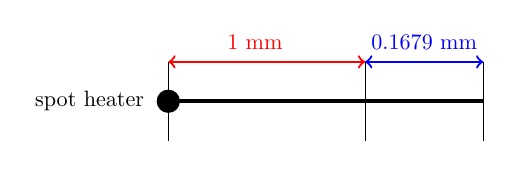
\begin{tikzpicture}[scale = 1]

\filldraw [black] (0,0) circle (4pt);
\draw [ultra thick] (0.0,0.0) -- (4.0,0);

\draw [thin] (2.5,-0.5) -- (2.5,0.5);
\draw [thin] (4.0,-0.5) -- (4.0,0.5);
\draw [thin] (0.0,-0.5) -- (0.0,0.5);

\draw [thick, <->, red] (0.0,0.5) -- (2.5,0.5);
\draw [thick, <->, blue] (2.5,0.5) -- (4.0,0.5);

\node[scale=0.8, color = black] at (-1.0,0.0) {spot heater};
\node[scale=0.8, color = red] at (1.1,0.75) {1 mm};
\node[scale=0.8, color = blue] at (3.25,0.75) {0.1679 mm};

\end{tikzpicture}
\caption{Schematic of 1D insulation modelling; simulation length as a sum of ground insulation (in red) and winding insulation (in blue) connected in series.}
\end{figure}


\clearpage